\documentclass[oneside]{book}
\usepackage{glossaries}
\usepackage{derivative}
\usepackage{pgfplots}
\usepackage{graphicx}
\usepackage{tikz}
\usepackage{float}
\usepackage{booktabs}
\usepackage{circuitikz}
\usepackage{amsmath}
\usepackage{fancyhdr}
\usepackage{amssymb}
\usepackage[list=true]{subcaption}
\usepackage{lastpage}
\usepackage{array}
\usepackage{hyperref}
\usepackage[a4paper,
    left=10mm,
    right=10mm,
    top=12mm,
    bottom=12mm,
]{geometry}
\setcounter{tocdepth}{3}
\newcolumntype{P}[1]{>{\centering\arraybackslash}p{#1}}
\begin{document}
\pagestyle{fancy}
    \fancyhf{}
\fancyhead[L]{EGB120 Foundations of Electrical Engineering}
\fancyhead[R]{\nouppercase{\leftmark}}
\fancyfoot[L]{Dinal Atapattu}
\renewcommand{\footrulewidth}{0.4pt}
\fancyfoot[R]{Page \thepage\ of \pageref{LastPage}}
    \title{
            Queensland University of Technology\\
            \rule{\linewidth}{0.5pt}
        \centering
        \textbf{EGB120} \\
        Foundations of Electrical Engineering\\
        \vspace{0.4cm}
        \rule{\linewidth}{1.5pt}
        \small{\textit{Professor Geoff Walker}}
    }
    \author{Dinal Atapattu}
    \date{\today}
    \maketitle
    \thispagestyle{empty}
    \tableofcontents
        \chapter{Electrical Circuits}
            \section{Fundamental Units}
                \begin{figure}[H]
                    \centering
                    \begin{tabular}{|p{0.15\textwidth}|p{0.4\textwidth}|p{0.15\textwidth}|p{0.15\textwidth}|}
                        \hline
                        \textbf{Quantity} & \textbf{Definition} & \textbf{Symbol} & \textbf{SI Unit} \\
                        \hline
                        Charge & Physical property of matter that causes it to experience a force
                        when placed in an electromagnetic field & $q$ & Coulomb (C) \\
                        \hline
                        Current & \begin{equation*}i(t) = \odv{q}{t}\end{equation*} & $i$ & Ampere (A) \\
                        \hline
                        Voltage & \begin{equation*}v(t) = \odv{w}{q}\end{equation*} & $v$ & Volt (V) \\
                        \hline
                        Power & \begin{equation*}p(t) = \odv{w}{t} = \odv{q}{t} \times \odv{w}{q} = vi \end{equation*} & $p$ & Watt (W) \\
                        \hline
                        Energy & \begin{equation*}w(\tau) = \int_{\tau}^{0} p(t) dt\end{equation*} & $e$ & Joule (J) \\
                        \hline
                    \end{tabular}
                \end{figure}
            \section{Basic Circuit Elements}
                \subsection{Voltage Source}
                    Produces or dissipates power at a specific voltage with whatever current is required
                \subsection{Current Source}
                    Produces or dissipates power at a specific current with whatever voltage is required
                \subsection{Resistor}
                    Dissipates power so that the voltage across the terminals is proportional to the current
                    \begin{align*}
                        v = Ri \tag{Ohm's Law}
                        \intertext{Following this}
                        p = vi = Ri^2 = \frac{v^2}{R}
                    \end{align*}
        \chapter{Simple Circuits}
            \section{Physics Ignored}
                \begin{itemize}
                    \item Electrical effects are instantaneous
                    \item Net charge on every component is zero
                    \item No magnetic coupling between components
                \end{itemize}
            \section{Series}
                Elements are connected end to end and \textbf{have the same current flowing through them}
                \begin{figure}[H]
                    \centering
                    \begin{circuitikz}
                        \draw (0,0) to[R=$R_1$] (2,0) to[R=$R_2$] (4,0) to[R=$R_3$] (6,0);
                    \end{circuitikz}
                    \caption{Series Circuit}
                \end{figure}
            \section{Parallel}
                Both ends of one element are connected directly and \textbf{have the same voltage across them}
                \begin{figure}[H]
                    \centering
                    \begin{circuitikz}
                        \draw (0,0) to[R=$R_1$] (0,2);
                        \draw (2,0) to[R=$R_2$] (2,2);
                        \draw (4,0) to[R=$R_3$] (4,2);
                        \draw (6,0) to[R=$R_4$] (6,2);
                        \draw (0,2) -- (6,2);
                        \draw (0,0) -- (6,0);
                    \end{circuitikz}
                    \caption{Parallel Circuit}
                \end{figure}
            \section{Kirchoff's Laws}
                \subsection{Kirchoff's Current Law}
                    The sum of currents entering a node is equal to the sum of currents leaving a node\\
                    \begin{minipage}{0.5\textwidth}
                        \begin{equation*}
                            \sum_{k=1}^{n} i_k = 0
                        \end{equation*}
                    \end{minipage}
                    \begin{minipage}{0.5\textwidth}
                        \begin{figure}[H]
                            \centering
                            \begin{circuitikz}
                                \draw (0,0) to[short, i=$i_1$] (2,0);
                                \draw (2,-2) to[short, i=$i_2$] (2,0);
                                \draw (4,0) to[short, i=$i_3$] (2,0);
                                \node at (2,0.7) {$i_1 + i_2 + i_3 = 0$};
                            \end{circuitikz}
                            \caption{Kirchoff's Current Law}
                        \end{figure}
                    \end{minipage}
                \subsection{Kirchoff's Voltage Law}
                    The sum of voltages around a closed loop is zero\\
                    \begin{minipage}{0.5\textwidth}
                        \begin{equation*}
                            \sum_{k=1}^{n} v_k = 0
                        \end{equation*}
                    \end{minipage}
                    \begin{minipage}{0.5\textwidth}
                        \begin{figure}[H]
                            \centering
                            \begin{circuitikz}[american]
                                \draw (0,2) to[battery, v_=$v_1$] (0,0);
                                \draw (0,2) to[short] (2,2);
                                \draw (2,2) to[resistor, l_=$R_1$, v^=$v_2$] (2,0);
                                \draw (2,0) to[resistor, l_=$R_2$, v^=$v_3$] (0,0);
                            \end{circuitikz}
                            \begin{align*}
                                v_1 - v_2 - v_3 &= 0\\
                                v_1 &= v_2 + v_3
                            \end{align*}
                            \caption{Kirchoff's Voltage Law}
                        \end{figure}
                    \end{minipage}
            \section{Component Behaviours in Series and Parallel}
                \begin{figure}[H]
                    \centering
                    \begin{tabular}{p{0.15\textwidth} p{0.25\textwidth} p{0.25\textwidth}}
                        \hline
                        \textbf{Component} & \textbf{Series} & \textbf{Parallel} \\
                        \hline
                        Voltage Source & $v_s = v_1 + v_2 + v_3$ & $v_s = v_1 = v_2 = v_3$\\
                        \hspace{0.2cm}\\
                        Current Source & $i_s = i_1 = i_2 = i_3$ & $i_s = i_1 + i_2 + i_3$\\
                        \hspace{0.2cm}\\
                        Resistor & $R_s = R_1 + R_2 + R_3$ & $\frac{1}{R_s} = \frac{1}{R_1} + \frac{1}{R_2} + \frac{1}{R_3}$\\
                        \hspace{0.2cm}\\
                        Inductor & $L_s = L_1 + L_2 + L_3$ & $\frac{1}{L_s} = \frac{1}{L_1} + \frac{1}{L_2} + \frac{1}{L_3}$\\
                        \hspace{0.2cm}\\
                        Capacitor & $\frac{1}{C_s} = \frac{1}{C_1} + \frac{1}{C_2} + \frac{1}{C_3}$ & $C_s = C_1 + C_2 + C_3$\\
                        \hspace{0.2cm}\\
                        \hline
                    \end{tabular}
                    \caption{Component Behaviours in Series and Parallel}
                \end{figure}
            \section{Voltage Divider}
                \begin{minipage}{0.6\linewidth}
                    \begin{figure}[H]
                        \centering
                        \begin{circuitikz}[american]
                            \draw (0,0) to[battery, v_=$v_s$, invert] (0,4);
                            \draw (0,4) to[short] (2,4);
                            \draw (2,4) to[resistor, l_=$R_1$, v^=$v_1$] (2,2);
                            \draw (2,2) to[resistor, l_=$R_2$, v^=$v_2$] (2,0);
                            \draw (2,0) to[short] (0,0);
                            \draw (2,2) to[short] (4,2); 
                            \draw (2,0) to[short] (4,0); 
                        \end{circuitikz}
                        \caption{Voltage Divider}
                    \end{figure} 
                \end{minipage}
                \begin{minipage}{0.3\linewidth}
                    \begin{flalign*}
                        \intertext{Current through resistors is}
                        i &= \frac{v_s}{R_1 + R_2}\\
                        \intertext{Voltage across resistors is}
                        v_1 &= iR_1 = \frac{R_1}{R_1 + R_2}v_s\\
                        \intertext{For more resistors}
                        v_k &= \frac{R_j}{R_{eq}}v_s
                    \end{flalign*}
                \end{minipage}
            \section{Current Divider}
                \begin{minipage}{0.6\linewidth}
                    \begin{figure}[H]
                        \centering
                        \begin{circuitikz}[american]
                            \draw (0,0) to[current source, v^=$i$] (0,2);
                            \draw (2,2) to[resistor, l_=$R_1$, i^=$i_1$] (2,0);
                            \draw (4,2) to[resistor, l_=$R_2$, i^=$i_2$] (4,0);
                            \draw (6,2) to[resistor, l_=$R_3$, i^=$i_3$] (6,0);
                            \draw (0,0) to[short] (6,0);
                            \draw (0,2) to[short] (6,2);
                        \end{circuitikz}
                        \caption{Current Divider}
                    \end{figure} 
                \end{minipage}
                \begin{minipage}{0.3\linewidth}
                    \begin{flalign*}
                        \intertext{Voltage across resistors is}
                        v &= i(R_1 || R_2 || R_3)\\
                        \intertext{Current through resistors is}
                        i_j &= \frac{v}{R_j} = \frac{R_1 || R_2 || R_3}{R_j}i\\
                        \intertext{For more resistors}
                        i_j &= \frac{R_{eq}}{R_{j}}i
                    \end{flalign*}
                \end{minipage}
        \chapter{Diodes}
            Current flows from the anode to the cathode and the voltage across the diode is positive.\\
            A diode requires voltage to be applied across it to conduct current. This voltage is called the \textbf{forward voltage}.
            \section{Voltage-Current Characteristics}
                \begin{figure}[htbp]
                    \centering
                    \begin{subfigure}{0.3\textwidth}
                        \centering
                        \begin{tikzpicture}
                            \begin{axis}[
                                xlabel={Voltage (V)},
                                ylabel={Current (A)},
                                title={Resistor},
                                width=\linewidth,
                                height=\linewidth,
                                xmin=-1, xmax=11,
                                ymin=-1, ymax=11,
                                xtick={0, 5, 10},
                                ytick={0, 5, 10},
                            ]
                            \addplot[domain=0:10, samples=100, color=red]{x};
                            \end{axis}
                        \end{tikzpicture}
                    \end{subfigure}
                    \begin{subfigure}{0.3\textwidth}
                        \centering
                        \begin{tikzpicture}
                            \begin{axis}[
                                xlabel={Voltage (V)},
                                ylabel={Current (A)},
                                title={Voltage Source},
                                width=\linewidth,
                                height=\linewidth,
                                xmin=-1, xmax=11,
                                ymin=-1, ymax=11,
                                xtick={0, 5, 10},
                                ytick={0, 5, 10},
                            ]
                            \addplot[domain=0:10, samples=100, color=red] coordinates {
                                (7, 0)
                                (7, 10)
                            };
                            \end{axis}
                        \end{tikzpicture}
                    \end{subfigure}
                    \begin{subfigure}{0.3\textwidth}
                        \centering
                        \begin{tikzpicture}
                            \begin{axis}[
                                xlabel={Voltage (V)},
                                ylabel={Current (A)},
                                title={Voltage Source},
                                width=\linewidth,
                                height=\linewidth,
                                xmin=-1, xmax=11,
                                ymin=-1, ymax=11,
                                xtick={0, 5, 10},
                                ytick={0, 5, 10},
                            ]
                            \addplot[domain=0:10, samples=100, color=red] coordinates {
                                (0, 7)
                                (10, 7)
                            };
                            \end{axis}
                        \end{tikzpicture}
                    \end{subfigure}
                    \caption{Diode VI Characteristics}
                \end{figure}
                \subsection{Simplified Diode Characteristics}
                    Diodes have non-linear characteristics. Therefore, they are simplified to make calculations easier.
                    \begin{figure}[H]
                        \centering
                        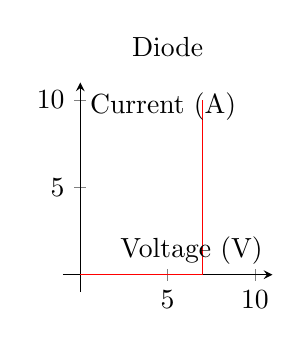
\begin{tikzpicture}
                            \begin{axis}[
                                xlabel={Voltage (V)},
                                ylabel={Current (A)},
                                title={Diode},
                                width=0.35\linewidth,  % Adjust the width to make the graph smaller
                                height=0.35\linewidth, % Adjust the height to make the graph smaller
                                xmin=-1, xmax=11,
                                ymin=-1, ymax=11,
                                xtick={0, 5, 10},
                                ytick={0, 5, 10},
                                axis lines=middle,   % Add x and y-axis lines
                            ]
                            \addplot[domain=0:10, samples=100, color=red] coordinates {
                                (0, 0)
                                (7, 0)
                                (7, 10)
                            };
                            \end{axis}
                        \end{tikzpicture}                        
                        \caption{Simplified Diode Characteristics}
                    \end{figure}
                \subsection{Full Diode Characteristics}
                    Diodes can be accurately modelled using Shcokley's equation
                    \begin{align*}
                        i_D = I_s \left( e^{\frac{v_D}{V_T} -1} \right) && V_T = \frac{kT}{q}
                    \end{align*}
                    where $I_s$ is the saturation current, $V_T$ is the thermal voltage, $k$ is Boltzmann's constant, $T$ is the temperature in Kelvin and $q$ is the charge of an electron.
            % \section{Operating Points}
            % \section{Load Lines}
        \chapter{RL and RC Circuits}
            \section{Natural Response}
                Is a decaying response for an RL and RC circuit
                \begin{figure}[H]
                    \centering
                    \begin{subfigure}{\linewidth}
                        \begin{equation*}
                            v(t) = V_0 e^{-\frac{t}{RC}}
                        \end{equation*}
                        \caption{Equation for RC Circuit Natural Response}
                    \end{subfigure}
                    \begin{subfigure}[t]{0.45\linewidth}
                        \centering
                        \begin{circuitikz}[american]
                            \draw (0,0)
                                to[capacitor, v=C, l=v, invert] (0,5)
                                to[short] (5,5)
                                to[resistor, R=R] (5,0)
                                to[short] (0,0);
                        \end{circuitikz}
                        \caption{Natural Response RC Circuit} 
                    \end{subfigure}
                    \begin{subfigure}[t]{0.45\linewidth}
                        \centering
                        \begin{tikzpicture}[scale=0.8]
                            \begin{axis}[
                                xlabel=$t$,
                                ylabel=$v$,
                                legend style={nodes={scale=0.8, transform shape}},
                            ]
                            \addplot[blue, domain=0:5] {5*exp(-x)};
                            \end{axis}
                        \end{tikzpicture}
                        \caption{VT Curve for RC Circuit Natural Response}
                    \end{subfigure}
                    \caption{RC Natural Response}
                \end{figure}
                \begin{figure}[H]
                    \centering
                    \begin{subfigure}{\linewidth}
                        \begin{equation*}
                            i(t) = I_0 e^{-\frac{Rt}{L}}
                        \end{equation*}
                        \caption{Equation for RL Circuit Natural Response}
                    \end{subfigure}
                    \begin{subfigure}[t]{0.45\linewidth}
                        \centering
                        \begin{circuitikz}[american]
                            \draw (0,0)
                                to[inductor, v=L, l=i, invert] (0,5)
                                to[short] (5,5)
                                to[resistor, R=R] (5,0)
                                to[short] (0,0);
                        \end{circuitikz}
                        \caption{Natural Response RL Circuit} 
                    \end{subfigure}
                    \begin{subfigure}[t]{0.45\linewidth}
                        \centering
                        \begin{tikzpicture}[scale=0.8]
                            \begin{axis}[
                                xlabel=$t$,
                                ylabel=$i$,
                                legend style={nodes={scale=0.8, transform shape}},
                            ]
                            \addplot[blue, domain=0:5] {5*exp(-x)};
                            \end{axis}
                        \end{tikzpicture}
                        \caption{VT Curve for RL Circuit Natural Response}
                    \end{subfigure}
                    \caption{RL Natural Response}
                \end{figure}
            \section{Step Response}
                \begin{figure}[H]
                    \centering
                    \begin{subfigure}{\linewidth}
                        \begin{equation*}
                            v(t) = I_sR + (V_0 - I_sR)e^{-\frac{t}{RC}}
                        \end{equation*}
                        \caption{Equation for RC Circuit Step Response}
                    \end{subfigure}
                    \begin{subfigure}{0.45\linewidth}
                        \begin{circuitikz}[american]
                            \draw (0,0)
                                to[current source, I=$I_s$] (0,5)
                                to[short] (3,5)
                                to[switch, l=$\text{t=0}$] (5,5)
                                to[capacitor, l=C, invert] (5,0)
                                to[short] (0,0);
                            \draw (2.5, 5)
                                to[resistor, R=R] (2.5, 0) node[ground]{};
                        \end{circuitikz}
                        \caption{Step Response RC Circuit}
                    \end{subfigure}
                    \begin{subfigure}{0.45\linewidth}
                        \begin{tikzpicture}[scale=0.8]
                            \begin{axis}[
                                xlabel=$t$,
                                ylabel=$v$,
                                legend style={nodes={scale=0.8, transform shape}},
                            ]
                                \addplot[blue, domain=0:5] {5 - 5*exp(-x)};
                            \end{axis}
                        \end{tikzpicture}
                        \caption{VT Curve for RC Circuit Step Response}
                    \end{subfigure}
                    \caption{RC Step Response}
                \end{figure}
                \begin{figure}[H]
                    \centering
                    \begin{subfigure}{\linewidth}
                        \begin{equation*}
                            i(t) = \frac{V_s}{R} + \left(I_o - \frac{V_s}{R}\right)e^{-\frac{Rt}{L}}
                        \end{equation*}
                        \caption{Equation for RL Circuit Step Response}
                    \end{subfigure}
                    \begin{subfigure}{0.45\linewidth}
                        \begin{circuitikz}[american]
                            \draw (0,0)
                                to[voltage source, v=$V_s$] (0,5)
                                to[short] (3,5)
                                to[switch, l=$\text{t=0}$] (5,5)
                                to[inductor, l=L, invert] (5,0)
                                to[short] (0,0);
                        \end{circuitikz}
                        \caption{Step Response RL Circuit}
                    \end{subfigure}
                    \begin{subfigure}{0.45\linewidth}
                        \begin{tikzpicture}[scale=0.8]
                            \begin{axis}[
                                xlabel=$t$,
                                ylabel=$i$,
                                legend style={nodes={scale=0.8, transform shape}},
                            ]
                                \addplot[blue, domain=0:5] {5 - 5*exp(-x)};
                            \end{axis}
                        \end{tikzpicture}
                        \caption{VT Curve for RL Circuit Step Response}
                    \end{subfigure}
                    \caption{RL Step Response}
                \end{figure}
        \chapter{AC}
            \section{AC Circuit Analysis}
                \begin{figure}[H]
                    \centering
                    \begin{tabular}{ccc}
                        \textbf{Element} & \textbf{Impedance} & \textbf{Diagram}\\
                        \toprule
                        Resistor & $R$ & \begin{circuitikz}[american]
                            \draw (0,0) to[resistor] (2,0);\end{circuitikz}\\
                        Capacitor & $\frac{1}{j\omega C}$ or $\omega L \angle 90^{\circ}$ & \begin{circuitikz}[american] \draw (0,0) to[capacitor, l=C] (2,0);\end{circuitikz}\\
                        Inductor & $j\omega L$ or $\frac{1}{\omega L} \angle -90^{\circ}$ & \begin{circuitikz}[american] \draw (0,0) to[inductor, l=L] (2,0);\end{circuitikz}\\
                    \end{tabular}
                    \caption{Impedance of Circuit Elements}
                \end{figure}
            \section{Bode Plots}
                Plot frequency on x axis using the log of frequency
                \begin{itemize}
                    \item 1, 10, 100, 1000, 10000 are equally spaced
                    \item 3, 30, 300, 3000, 30000 are midpoints
                \end{itemize}
                Plot the log of gain (decibels) on one y axis and the phase (degrees) on another y axis
                \begin{figure}[H]
                    \centering
                    \begin{subfigure}{0.22\linewidth}
                        \centering
                        \begin{align*}
                            \omega = 2\pi f\\\\
                        \end{align*}
                        \caption{Hz to Radians per Second}
                    \end{subfigure}
                    \begin{subfigure}{0.22\linewidth}
                        \centering
                        \begin{align*}
                            \text{Gain}_{\text{dB}} = 20\log_{10}\left(\text{Gain}\right)\\\\
                        \end{align*}
                        \caption{Gain to Decibels}
                    \end{subfigure}
                    \begin{subfigure}{0.22\linewidth}
                        \centering
                        \begin{align*}
                            H(\omega) = \frac{V_o(\omega)}{V_i(\omega)}\\\\
                        \end{align*}
                        \caption{Transfer Function}
                    \end{subfigure}
                    \begin{subfigure}{0.22\linewidth}
                        \centering
                        \begin{align*}
                            \text{Phase} &= \angle H(\omega)\\
                            &= \arctan \frac{\text{imag} (H(\omega))}{\text{real} (H(\omega))}
                        \end{align*}
                        \caption{Transfer Function to Phase}
                    \end{subfigure}
                    \begin{subfigure}{0.22\linewidth}
                        \centering
                        \begin{align*}
                            \text{Gain} &= \left|(H(\omega))\right|\\
                            &= \sqrt{\left(\text{real} (H(\omega))\right)^2 + \left(\text{imag} (H(\omega))\right)^2}
                        \end{align*}
                        \caption{Transfer Function to Gain}
                    \end{subfigure}
                    \caption{Bode Plot Equations}
                \end{figure}
            \section{Transfer Function $H(\omega)$ - The 3dB Point}
                The 3dB point is the frequency at which the gain is $\frac{1}{\sqrt{2}}$ of the maximum gain.
                Also called the \textbf{half power point} or \textbf{half power frequency} or \textbf{break frequency} or \textbf{corner frequency}
        \chapter{Filters and Rectifiers}
            Filters keep the desired frequency components of a signal and remove the unwanted frequency components.\\
            They do this in the frequency domain
            \section{Applications of Filters}
                \begin{itemize}
                    \item Audio Signals
                    \begin{itemize}
                        \item Remove high frequency hiss (magnetic tape)
                        \item Remove low frequency rumble (vinyl)
                    \end{itemize}
                    \item Medical Signals
                    \begin{itemize}
                        \item EEG alpha waves are 8-12Hz
                        \item EEG beta waves are 12-30Hz
                        \item ECG waves are 1 - 40Hz
                    \end{itemize}
                    \item 50Hz interference
                    \begin{itemize}
                        \item Remove all signals near 50Hz
                    \end{itemize}
                    \item Signal Processing
                \end{itemize}
            \section{Ideal Filters}
                \begin{figure}[H]
                    \centering
                    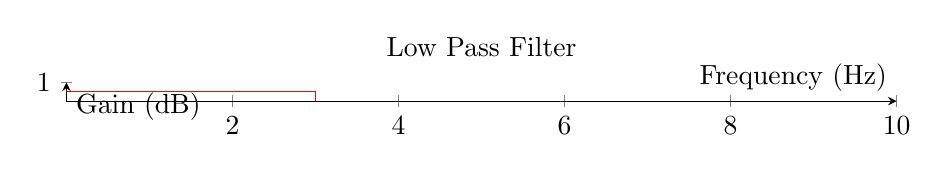
\begin{tikzpicture}
    \begin{axis}[
        xlabel={Frequency (Hz)},
        ylabel={Gain (dB)},
        title={Low Pass Filter},
        width=\linewidth,
        height=0.15\linewidth,
        xmin=0, xmax=10,
        ymin=0, ymax=1,
        ytick={1},
        xtick={0, 2, 4, 6, 8, 10},
        axis lines=middle,
    ]
    \addplot[domain=0:10, samples=100, color=red] coordinates {
        (0, 0.5)
        (3, 0.5)
        (3, 0)
    };
    \end{axis}
\end{tikzpicture}
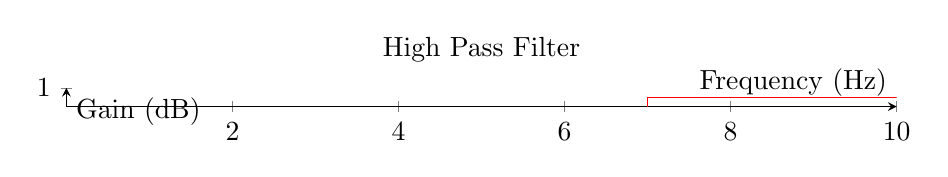
\begin{tikzpicture}
    \begin{axis}[
        xlabel={Frequency (Hz)},
        ylabel={Gain (dB)},
        title={High Pass Filter},
        width=\linewidth,
        height=0.15\linewidth,
        xmin=0, xmax=10,
        ymin=0, ymax=1,
        ytick={1},
        xtick={0, 2, 4, 6, 8, 10},
        axis lines=middle,
    ]
    \addplot[domain=0:10, samples=100, color=red] coordinates {
        (7, 0)
        (7, 0.5)
        (10, 0.5)
    };
    \end{axis}
\end{tikzpicture}
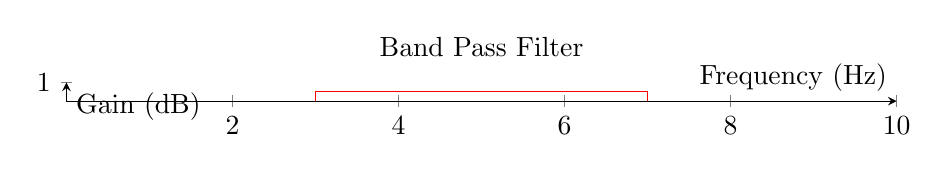
\begin{tikzpicture}
    \begin{axis}[
        xlabel={Frequency (Hz)},
        ylabel={Gain (dB)},
        title={Band Pass Filter},
        width=\linewidth,
        height=0.15\linewidth,
        xmin=0, xmax=10,
        ymin=0, ymax=1,
        ytick={1},
        xtick={0, 2, 4, 6, 8, 10},
        axis lines=middle,
    ]
    \addplot[domain=0:10, samples=100, color=red] coordinates {
        (3, 0)
        (3, 0.5)
        (7, 0.5)
        (7, 0)
    };
    \end{axis}
\end{tikzpicture}
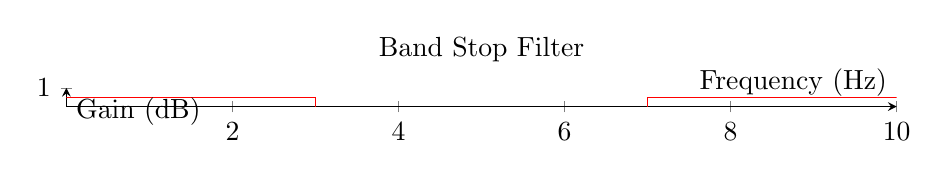
\begin{tikzpicture}
    \begin{axis}[
        xlabel={Frequency (Hz)},
        ylabel={Gain (dB)},
        title={Band Stop Filter},
        width=\linewidth,
        height=0.15\linewidth,
        xmin=0, xmax=10,
        ymin=0, ymax=1,
        ytick={1},
        xtick={0, 2, 4, 6, 8, 10},
        axis lines=middle,
    ]
     \addplot[domain=0:10, samples=100, color=red] coordinates {
        (0, 0.5)
        (3, 0.5)
        (3, 0)
    };
    \addplot[domain=0:10, samples=100, color=red] coordinates {
        (7, 0)
        (7, 0.5)
        (10, 0.5)
    };
    \end{axis}
\end{tikzpicture}
                    \caption{Ideal Filters}
                \end{figure}
            \section{Passive Filters}
                \subsection{Low Pass Filter}
                    \begin{figure}[H]
                        \centering
                        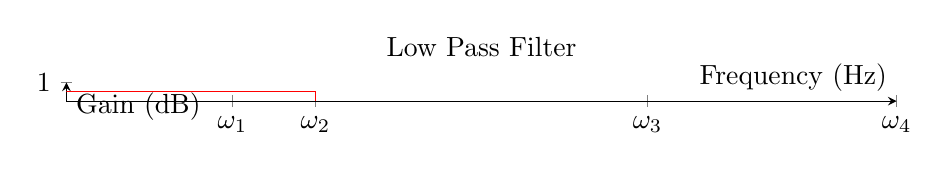
\begin{tikzpicture}
    \begin{axis}[
        xlabel={Frequency (Hz)},
        ylabel={Gain (dB)},
        title={Low Pass Filter},
        width=\linewidth,
        height=0.15\linewidth,
        xmin=0, xmax=10,
        ymin=0, ymax=1,
        ytick={1},
        xtick={0, 2, 3, 7, 10},
        xticklabels={0, $\omega_1$, $\omega_2$, $\omega_3$, $\omega_4$, $\omega_5$},
        axis lines=middle,
    ]
    \addplot[domain=0:10, samples=100, color=red] coordinates {
        (0, 0.5)
        (3, 0.5)
        (3, 0)
    };
    \end{axis}
\end{tikzpicture}
                        \caption{Low Pass Filter}
                    \end{figure}
                    \begin{figure}[H]
                        \centering
                        \begin{circuitikz}[american]
                            \draw (0,0) to[voltage source, v=$v_i\left(\omega\right)$, invert] (0,2);
                            \draw (0,2) to[short] (2,2);
                            \draw (2,2) to[resistor, l^=$1\text{k}\Omega$] (4,2);
                            \draw (4,2) to[capacitor, l^=$1\mu $F] (4,0);
                            \draw (4,0) to[short] (0,0);
                            \draw (4,2) to[short] (6,2);
                            \draw (4,0) to[short] (6,0);
                            \draw (6,1) node[right] {$v_o\left(\omega\right)$};
                            \draw[dotted] (2,-1) rectangle (5.5,3);
                        \end{circuitikz}
                    \end{figure}
                    \begin{align*}
                        v_o(\Omega) &= \frac{\frac{1}{j\omega C}}{R + \frac{1}{j\omega C}}v_i(\omega)\\
                        \frac{v_0 (\omega)}{v_i (\omega)} &= \frac{1}{j\omega RC + 1}\\
                        \intertext{For $R = 1\text{k}\Omega$ and $C = 1\mu F$}
                        H(\omega) &= \frac{1000}{j\omega + 1000}\\
                        H(62.8) \approx 1 && H(62800) = 0.016 \angle -89^{\circ}
                    \end{align*}
                    \subsubsection{Plotting the Response}
                        \begin{figure}[H]
                            \centering
                            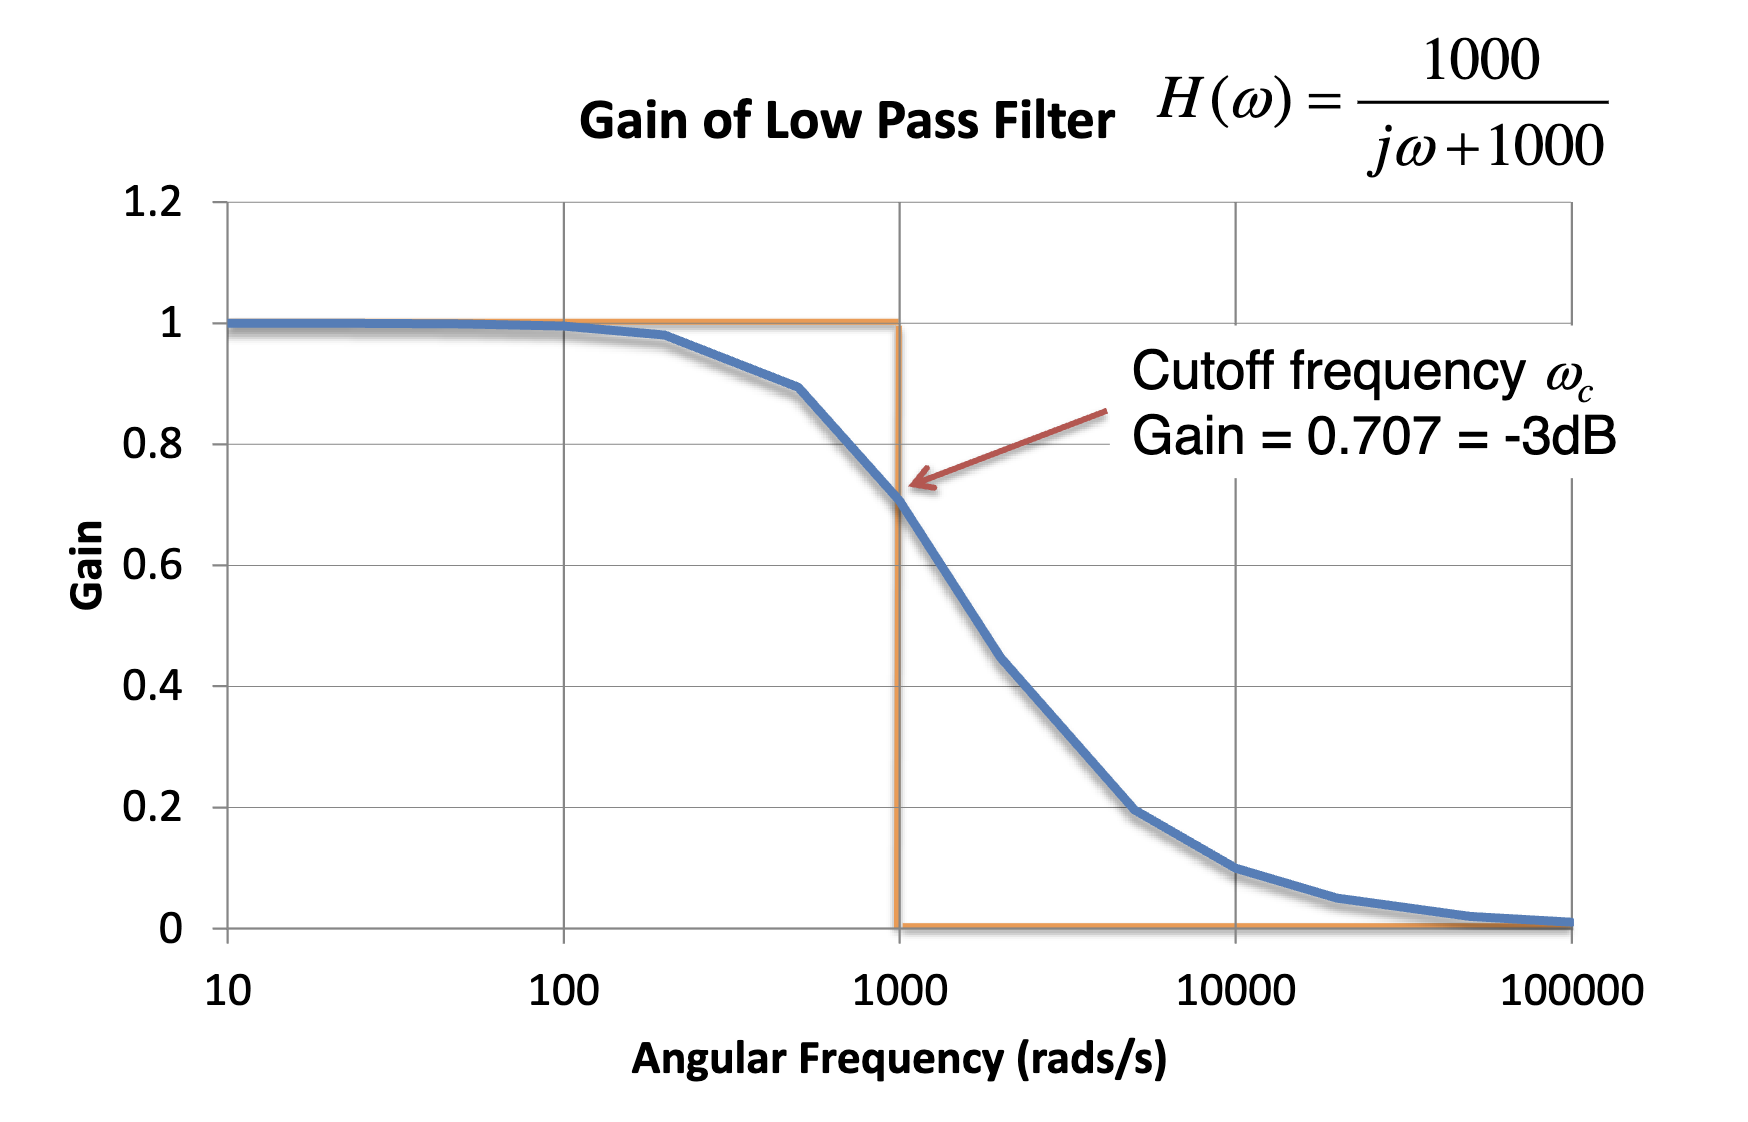
\includegraphics[width=0.5\linewidth]{figures/lowpass_bode.png}
                            \caption{Low Pass Filter Bode Plot}
                        \end{figure}
                    \subsubsection{Desigining a Low Pass Filter}
                        Find the required \textbf{cutoff frequency} $\omega_c$ in radians per second (remember $\omega_c = 2\pi f$)\\
                        Choose a value for $R$ and calculate $C$ such that $\omega_c = \frac{1}{RC}$\\
                        \begin{minipage}{0.5\linewidth}
                            \begin{figure}[H]
                                \centering
                                \begin{circuitikz}[american]
                                    \draw (0,0) to[voltage source, v=$v_i\left(\omega\right)$, invert] (0,2);
                                    \draw (0,2) to[short] (2,2);
                                    \draw (2,2) to[resistor, l^=R] (4,2);
                                    \draw (4,2) to[capacitor, l^=C] (4,0);
                                    \draw (4,0) to[short] (0,0);
                                    \draw (4,2) to[short] (6,2);
                                    \draw (4,0) to[short] (6,0);
                                    \draw (6,1) node[right] {$v_o\left(\omega\right)$};
                                    \draw[dotted] (2,-1) rectangle (5.5,3);
                                \end{circuitikz}
                            \end{figure}
                        \end{minipage}
                        \begin{minipage}{0.5\linewidth}
                            \begin{align*}
                                H(\omega) &= \frac{\frac{1}{RC}}{j\omega + \frac{1}{RC}}\\
                                \omega_c &= \frac{1}{RC}
                            \end{align*} 
                        \end{minipage}
                \subsection{High Pass Filter}
                    Similar to a low pass filter, but the capacitor and resistor are swapped\\
                    \subsubsection{Desigining a High Pass Filter}
                        \begin{minipage}{0.5\linewidth}
                            \begin{figure}[H]
                                \centering
                                \begin{circuitikz}[american]
                                    \draw (0,0) to[voltage source, v=$v_i\left(\omega\right)$, invert] (0,2);
                                    \draw (0,2) to[short] (2,2);
                                    \draw (2,2) to[capacitor, l^=C] (4,2);
                                    \draw (4,2) to[resistor, l^=R] (4,0);
                                    \draw (4,0) to[short] (0,0);
                                    \draw (4,2) to[short] (6,2);
                                    \draw (4,0) to[short] (6,0);
                                    \draw (6,1) node[right] {$v_o\left(\omega\right)$};
                                    \draw[dotted] (2,-1) rectangle (5.5,3);
                                \end{circuitikz}
                            \end{figure}
                        \end{minipage}
                        \begin{minipage}{0.5\linewidth}
                            \begin{align*}
                                v_o(\omega) &= \frac{R}{R + \frac{1}{j\omega C}}v_i(\omega)\\
                                \frac{v_0 (\omega)}{v_i (\omega)} = H(\omega) &= \frac{j\omega RC}{j\omega RC + 1}\\\\
                                \omega_c &= \frac{1}{RC}
                            \end{align*}
                        \end{minipage}
                    \subsubsection{Plotting the Response}
                        \begin{figure}[H]
                            \centering
                            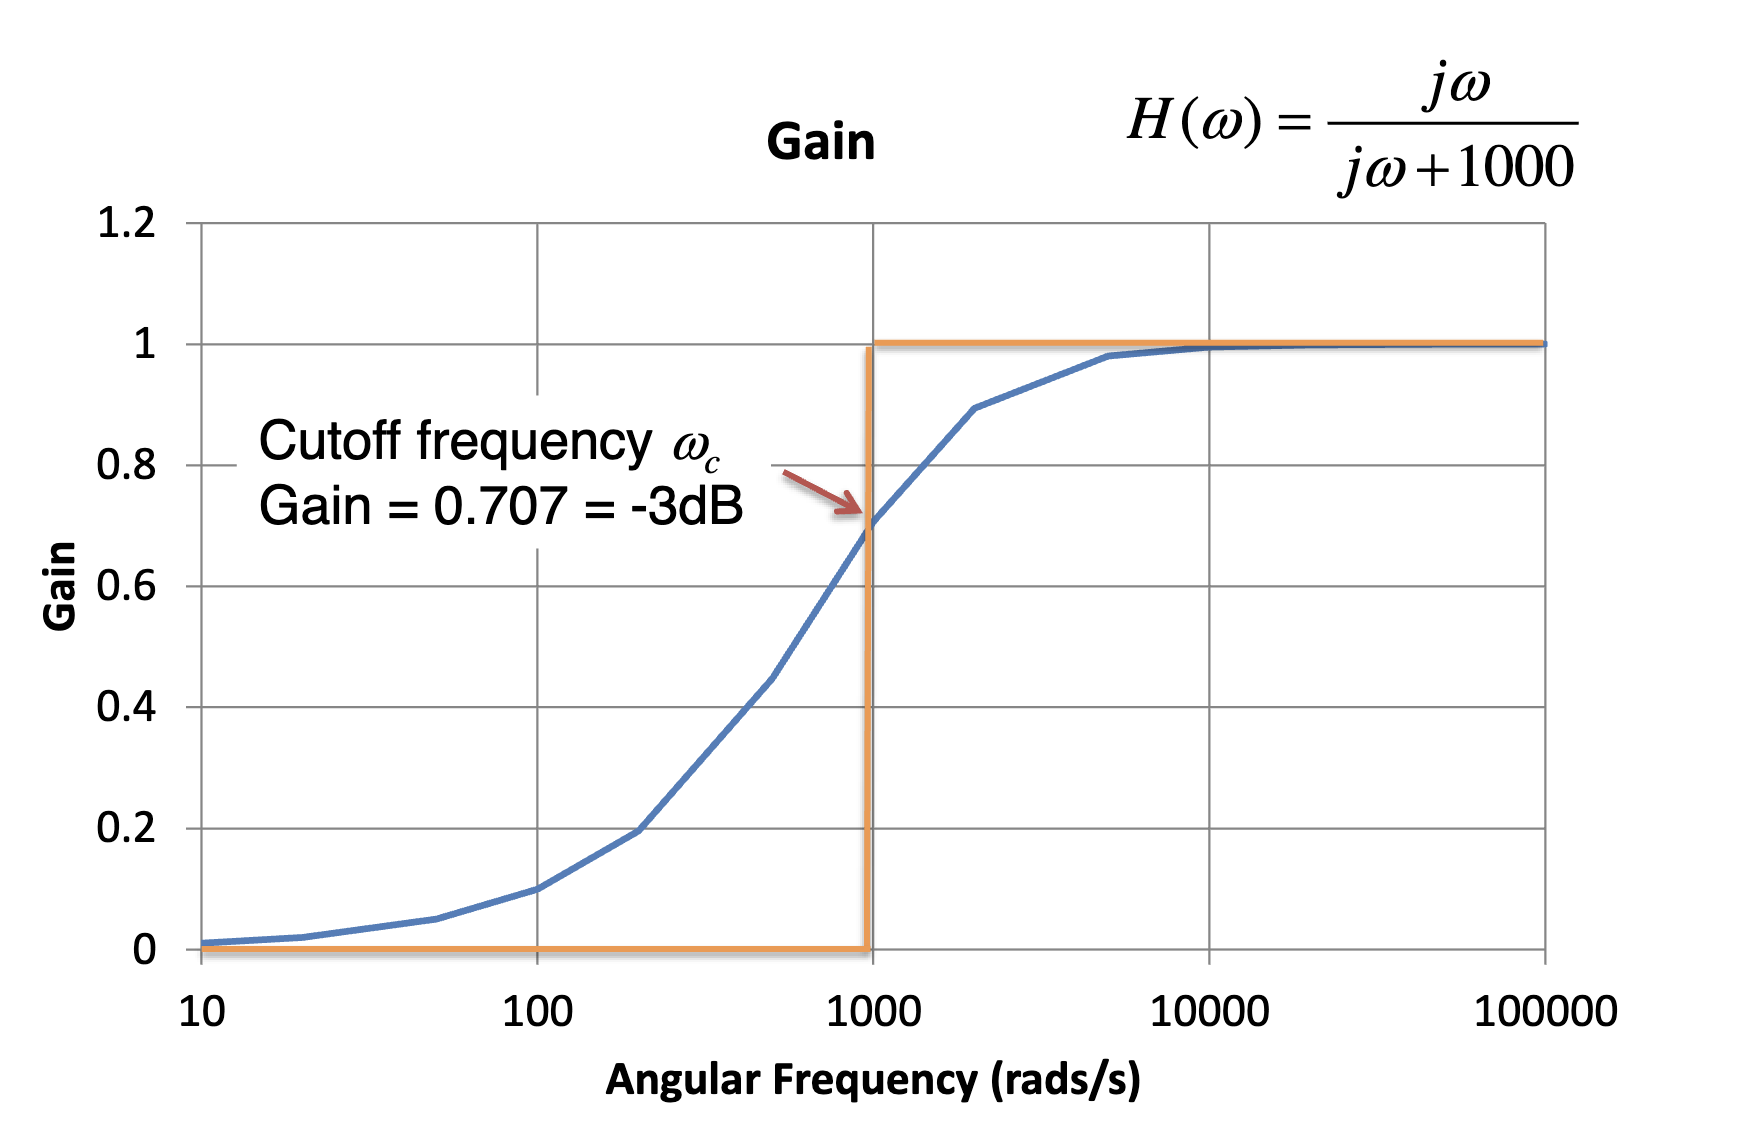
\includegraphics[width=0.5\linewidth]{figures/highpass_bode.png}
                            \caption{High Pass Filter Bode Plot}
                        \end{figure}
            \section{Active Filters}
                \subsection{Op-Amps}
                    \begin{figure}[H]
                        \begin{subfigure}{0.45\linewidth}
                            \centering
                            \begin{circuitikz}[american]
                                \draw (0,0) node[op amp] (opamp) {};
                                \node[above] at (-3,0.7) {$v_{in}$};
                                \draw (-3,0.5) to[resistor, R=$Z_1$] (opamp.-);
                                \draw (opamp.-) to[short] ++(0,1) to[short] ++(0.5,0) to[resistor, R=$Z_2$] ++(3,0) to[short] ++(0,-1.5);
                                \draw (opamp.out) to[short] ++(2,0) node[right] {$v_o$};
                                % ground
                                \draw (opamp.+) to[short] ++(-0.5,0) to[short] ++(0,-0.5) node[ground] {};
                            \end{circuitikz}
                            \subcaption{Inverting Amplifier}
                        \end{subfigure}
                        \begin{subfigure}{0.45\linewidth}
                            \centering
                            \begin{circuitikz}[american]
                                \draw (0,0) node[op amp, noinv input up] (opamp) {};
                                \node[above] at (-3,0.7) {$v_{in}$};
                                \draw (-3,0.5) to[short] (opamp.+);
                                \draw (opamp.-) to[short] ++(0,-1) to[resistor, R=$Z_1$] ++(-2,0) node[ground] {};
                                \draw (opamp.out) to[short] ++(0,-1.5) to[resistor, R=$Z_2$] ++(-2.38,0);
                                \draw (opamp.out) to[short] ++(2,0) node[right, R=$Z_3$] {$v_o$};
                            \end{circuitikz}
                            \subcaption{Non-Inverting Amplifier}
                        \end{subfigure}
                        \caption{Active Filters}
                    \end{figure}
                \subsection{Using an Op Amp}
                    \subsubsection{Active High Pass Filter}
                        \begin{minipage}{0.7\linewidth}
                            \begin{figure}[H]
                                \centering
                                \begin{circuitikz}[american]
                                    \draw (0,0) node[op amp] (opamp) {};
                                    \draw (-4.5, 0.5) to [capacitor, l_=$1\mu$F] ++(1.5,0);
                                    \node[above] at (-5,0.7) {$v_{in}$};
                                    \draw (-3,0.5) to[resistor, l=$1\text{k}\Omega$] (opamp.-);
                                    \draw (opamp.-) to[short] ++(0,1) to[short] ++(0.5,0) to[resistor, l=$10\text{k}\Omega$] ++(3,0) to[short] ++(0,-1.5);
                                    \draw (opamp.out) to[short] ++(2,0) node[right] {$v_o$};
                                    % ground
                                    \draw (opamp.+) to[short] ++(-0.5,0) to[short] ++(0,-0.5) node[ground] {};
                                    \draw[dotted, thick] (-4.5, -0.5) rectangle (-1.25, 1.5) node[above] at (-3.25, 1.5) {$Z_1$};
                                    \draw[dotted, thick] (-1, 1) rectangle (2.25, 2.5) node[above] at (0.625, 2.5) {$Z_2$};
                                \end{circuitikz}
                                \subcaption{Active High Pass Filter}
                            \end{figure}
                        \end{minipage}
                        \begin{minipage}{0.3\linewidth}
                            \begin{align*}
                                v_o &= -\frac{Z_2}{Z_1}v_{in}\\
                                \frac{v_o}{v_{in}} &= -\frac{R_2}{R_1 + \frac{1}{j\omega C_1}} = -\frac{R_2}{R_1} \frac{j\omega}{j\omega + \frac{1}{R_1 C_1}}\\
                            \end{align*}
                            High pass filter with\\
                            $\omega_c = \frac{1}{R_1 C_1} = \frac{1}{10^3 \times 10^{-6}} = 1000\text{rad/s}$\\\\
                            Gain of $-\frac{R_2}{R_1} = -10$ in passband
                        \end{minipage}
                    \subsubsection{Active Low Pass Filter}
                        \begin{minipage}{0.7\linewidth}
                            \begin{figure}[H]
                                \centering
                                \begin{circuitikz}[american]
                                    \draw (0,0) node[op amp] (opamp) {};
                                    \node[above] at (-3.5,0.7) {$v_{in}$};
                                    \draw (-3.5,0.5) to[resistor, R=1k$\Omega$] (opamp.-);
                                    \draw (opamp.-) to[short] ++(0,1) to[resistor, R=10k$\Omega$]++(3,0) to[short] ++(0,-1.5);
                                    \draw (opamp.-) to[short] ++(0,2.5) to[capacitor, C=$1\mu$F] ++(3,0) to[short] ++(0,-3);
                                    \draw (opamp.out) to[short] ++(2,0) node[right] {$v_o$};
                                    % ground
                                    \draw (opamp.+) to[short] ++(-0.5,0) to[short] ++(0,-0.5) node[ground] {};
                                    \draw[dotted, thick] (-3, 0) rectangle (-1.5, 1.5) node[above] at (-2.25, 1.5) {$Z_1$};
                                    \draw[dotted, thick] (-0.5, 1) rectangle (1, 4) node[above] at (0.25, 4) {$Z_2$};
                                \end{circuitikz}
                                \subcaption{Active Low Pass Filter}
                            \end{figure}
                        \end{minipage}
                        \begin{minipage}{0.3\linewidth}
                            \begin{align*}
                                v_o &= -\frac{Z_2}{Z_1}v_{in}\\
                                &= \frac{\frac{1}{\frac{1}{R_2} + j\omega C_2}}{R_1}v_{in}\\
                                \frac{v_o}{v_{in}} = H(\omega) &= -\frac{R_2}{R_1} \frac{1}{1+j\omega R_2C_2}\\
                                &= -\frac{R_2}{R_1} \frac{\frac{1}{R_2C_2}}{j\omega + \frac{1}{R_2C_2}}\\
                            \end{align*}
                            Low pass filter with \\$\omega_c = \frac{1}{R_2 C} = \frac{1}{10^4 \times 10^{-6}} = 100\text{rad/s}$\\\\
                            Gain of $-\frac{R_2}{R_1} = -10$ in passband
                        \end{minipage}
            \section{Band Pass and Band Stop Filters}
                \begin{figure}[H]
                    \centering
                    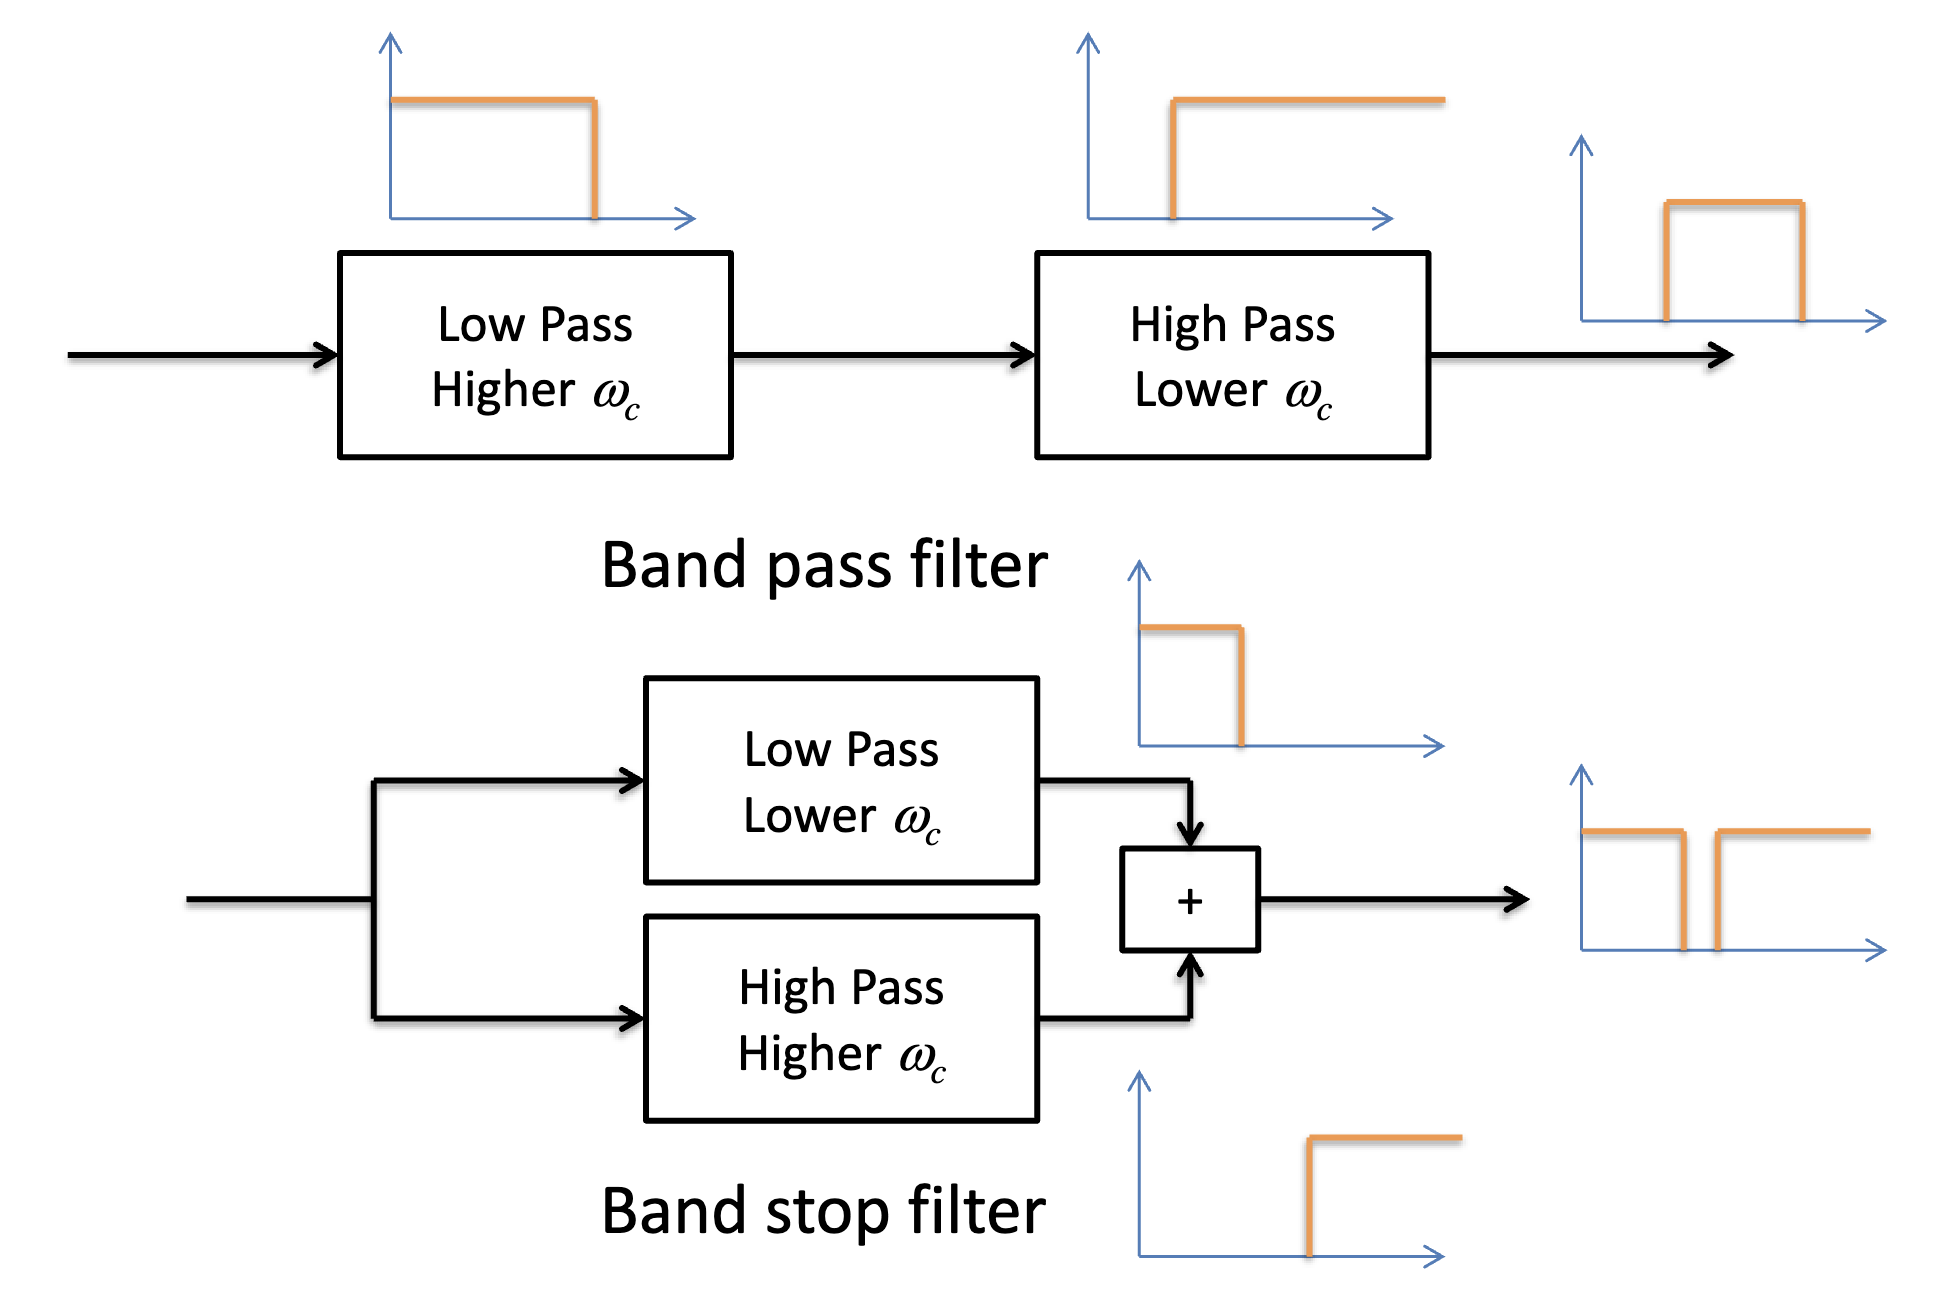
\includegraphics[width=0.6\linewidth]{figures/band_pass_stop.png}
                    \caption{Band Pass and Band Stop Filters}
                \end{figure}
        \listoffigures
        % \listoftables
\end{document}